A partir del diseño de la etapa de salida, se tiene el requerimiento de una corriente de al menos \SI{5}{\milli\ampere} para la polarización de la etapa amplificadora de tensión (VAS).

Se propone una etapa de emisor común con realimentación local ($RE = \SI{10}{\ohm}$), con lo cuál la ganancia de tensión es \eqref{ec.av_vas}. Siendo $R_{ca}$ la resistencia equivalente de la etapa de salida que puede aproximarse $\beta \cdot \beta \cdot R_L = 75 \cdot 60 \cdot \SI{8}{\ohm} = \SI{36}{\kilo\ohm}$

\begin{equation}
	\centering
	A_{v,vas} = \frac{-g_m \cdot R_{ca}}{1+g_m \cdot R_E} = 2400
	\label{ec.av_vas}
\end{equation}
	

Por otra parte la ganancia de tensión del comparador es

\begin{equation}
	\centering
	A_{v,pd} = \frac{-g_m \cdot R_ca}{1+g_m \cdot R_e} = \frac{-80mA/V \cdot \SI{36}{\kilo\ohm} }{ 1 + 80mA/V \cdot \SI{100}{\ohm} } = -13
	\label{ec.av_pd}
\end{equation}

Se propone una corriente de polarización para el par diferencial lo más pequeña posible con el fin de disminuir el ruido. Para contrarrestar la disminución de la ganancia se utilizó una reistencia de emisor $R_E=\SI{100}{\ohm}$.


La ganancia de tensión total queda determinada por la ganancia de la VAS y el comparador de entrada \eqref{ec-av_vas} y \eqref{av_pd} ya que la etapa de salida presenta una ganancia aproximadamente unitaria.

\begin{equation}
	\centering
	a = (-13) \cdot (-2400) = 31200
	\label{ec.a}
\end{equation}

Para una tensión de entrada de 1Vrms, se busca que la salida sea aproximadamente la máxima posible \SI{27}{\volt}, por lo que se propone una ganancia a lazo cerrado de 20, establecida por el bloque realimentador f.

\begin{equation}
	\centering
	f = \frac{RF1}{RF1 + RF2} = \frac{\SI{1.1}{\kilo\ohm}}{\SI{1.1}{\kilo\ohm} + \SI{22}{\kilo\ohm}} \approx 0,048
\end{equation}

\begin{equation}
	\centering
	af = 0,048 \cdot 31200 = 1485 \implies af >> 1 \implies A \approx \frac{1}{f} = 21
\end{equation}

\subsection{Resistencia de entrada}

\begin{itemize}
	
	\HgraficarEPS{0.5}{ri}{Diagrama en bloque para hallar la resistencia de entrada.}{fig.esq_ri}
		
	\item Resistencia de entrada sin realimentación
	
	\begin{equation}
		\centering
		R_{i,SR} = \SI{100}{\ohm} + R_{F1}//R_{F2} = \SI{100}{\ohm} + \SI{22}{\kilo\ohm}//\SI{1.1}{\kilo\ohm}
	\end{equation}
	
	\item Resistencia de entrada con realimentación
	\HgraficarEPS{0.5}{ri_realim}{Diagrama en bloque para hallar la resistencia de entrada.}{fig.esq_ri_f}
	\begin{equation}
		\centering
		R_{i,CR} = (1+ af) \cdot R_{i,SR} = (1 + 1485) \cdot \SI{1.1}{\kilo\ohm} = \SI{1.6}{\mega\hertz}
	\end{equation}
	
\end{itemize}

Finalmente la resistencia que ve el generador es

$$ \SI{100}{\kilo\ohm}//\SI{1.6}{\mega\hertz} = \boxed{\SI{94}{\kilo\ohm}} $$


\subsection{Impedancia de salida}

\begin{figure}[H]
	 \centering
	 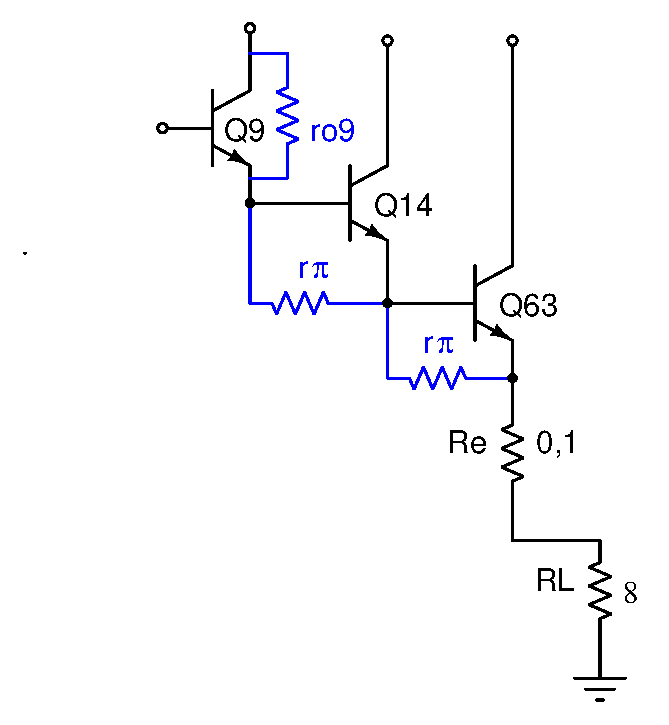
\includegraphics[scale=0.5]{ro.eps}
	 \caption{Diagrama para hallar la resistencia de salida del circuito sin realimentación.}
\end{figure}

\begin{itemize}
	\item Resistencia de salida sin realimentador: en esta situación se supone que, a los efectos de este cálculo, las resistencias de salida de los colectores comunes son iguales.
Entonces se calcula la resistencia de salida del circuito sin realimentar como
	\begin{equation}
		\centering
		R_o = \frac{1}{2} \cdot R_E + \frac{ r_{\pi}^{*} + r_{o,Q9} }{\beta^{*} } = \frac{1}{2} \left ( \SI{0.1}{\ohm} + \frac{\SI{32}{\kilo\ohm}}{75 \cdot 60} \right) = \SI{3.6}{\ohm},
	\end{equation}
	siendo
	\begin{equation}
		\centering
		r_{\pi}^{*} = 2 \cdot r_{\pi_Q14} = 2 \cdot 60 \cdot \frac{25mV}{ \SI{110}{\milli\ampere}} = \SI{14}{\ohm} 
	\end{equation}
		
	%\begin{equation}
	%	\centering
	%	r_{o,Q9} = \frac{160V}{5mA} = \SI{32}{\kilo\ohm}
	%\end{equation}
		
	\item Resistencia de salida con realimentador
	\begin{equation}
		\centering
		R_{o,CR} = \frac{R_{o,SR}}{1+ af} = \frac{ \SI{3.6}{\ohm} }{1+1485} = \boxed{\SI{2.4}{\milli\ohm}} 
	\end{equation}
\end{itemize}

\subsection{Factor de amortiguamiento}

En un sistema de audio, el factor de amortiguamiento es la relación entre la impedancia del altoparlante y la impedancia de salida del amplificador. Describe la capacidad del amplificador de controlar movimiento del altoparlante cuando se deja de excitarlo, en especial cercano a su frecuencia de resonancia. Este valor es de importancia en el contexto de las bajas frecuencias, o subwoofers, dado que la inercia de los diafragmas suele ser grande y el control de la suspensión débil, para permitir grandes excursiones.

\Flor{Debería ser mucho menor, 500 como mucho}
\begin{equation}
	\centering
	f_a= \frac{Z_L}{Z_o} = \frac{ \SI{8}{\ohm}}{ \SI{2.4}{\milli\ohm}}= \boxed{\num{3333}}
	\label{ec:fa}
\end{equation}



	
	






